\subsection{Results}
In training period, all possible patterns of each device are extracted and saved in the library $\mathbf{EDlib}$, in which pattern $j$ of device $i$ is denoted as 
\begin{equation}
f_{ij}^{ed} = \{\Delta x_{ij}^R,\Delta x_{ij}^F\},
\end{equation}
with notation $R$ for rising edge and $F$ for falling edge.
If the edge detector detects an event switched on at time $t_s$ and switched off at time $t_e$, the corresponding feature is
\begin{equation}
f^{ed} = \{\Delta x(t_s^1),\Delta x(t_e^{n_e})\}.
\end{equation}
The distance between two patterns $f_{ij}^{ed}$ and $f^{ed}$ can be calculated as
\begin{eqnarray}\label{eqED1}
\delta_{ij}^{ed} &=& d(f^{ed},f_{ij}^{ed})\nonumber \\
&=&|\Delta x(t_s^1)-\Delta x_{ij}^R|+|\Delta x(t_e^{n_e})-\Delta x_{ij}^F|.
\end{eqnarray}
In the ED algorithm, the detected event will be matched with the device having a pattern with the minimum distance. Nevertheless, in homes and buildings, there are several devices with the same edge height, which decreases the load disaggregation performance. To overcome this challenge, in SmartSense, the probability that each device $i, i=1,\ldots,N$, is turned on and off at the same time as the detected event, denoted as $p_i^R(t_s^1)$ and $p_i^F(t_e^{n_e})$, respectively, is estimated as in Section~\ref{model}. This means, $p_i^R(t_s^1)=(1-npv)$ if a rising edge of device $i$ is detected at time $t_s^1$ and $p_i^R(t_s^1)=(1-npv)$ on the contrary. Similarly, $p_i^F(t_e^{n_e})=pr$ if device $i$ has a falling edge at time $t_e^{n_e}$ and $p_i^F(t_e^{n_e})=(1-npv)$ on the contrary. In the case of unsupervised devices, $p_i^R(t_s^1) = p_i^F(t_e^{n_e}) = 0.5$. The coincidence probability that both edges appear is then
\begin{equation}\label{eqED2}
Pr_i^{ed} = p_i^R(t_s^1)\times p_i^F(t_e^{n_e}).
\end{equation}

To reduce the computational complexity, the multiplication in Eq.~\eqref{eqED2} can be transformed to an addition by applying the log-linear form, which gives
\begin{eqnarray}\label{eqED3}
\phi_i^{ed} &=& -\log{Pr_i^{ed}}\nonumber \\
&=& -\log{p_i^R(t_s^1)}-\log{p_i^F(t_e^{n_e})}.
\end{eqnarray}
The identified device does not only have a pattern with the minimum distance $\delta_{ij}^{ed}$, but also has the maximum probability $Pr_i^{ed}$, i.e. the minimum log-linear form $\phi_i^{ed}$. In other words, the ED algorithm will try to find the pattern giving the minimum modified distance, calculated as
\begin{eqnarray}
d_{ij}^{ed} = \delta_{ij}^{ed}+\lambda_1\times \phi_i^{ed},
\end{eqnarray}
where $\lambda_1$ is a regularization parameter. The load identification procedure for each detected pattern is presented in Algorithm~\ref{algo:ED1}, where $\Phi^{ed}$ contains the probability in log-linear form of all devices and $m_i$ denotes the number of patterns of device $i$ in $\mathbf{EDlib}$. The procedure is illustrated by a flowchart in Figure~\ref{fig:ed1}.
\begin{figure}[!h]
\centering
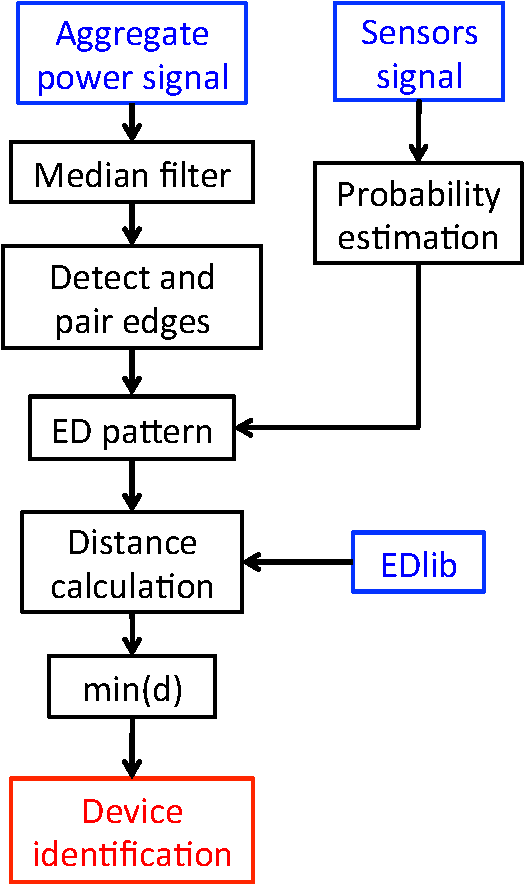
\includegraphics[width=0.45\textwidth]{./chapters/chapter4/images/EDschema.pdf} 
\caption{Load disaggregation based on the ED algorithm.} 
\label{fig:ed1} 
\end{figure}

\begin{algorithm}
\caption{Matching detected event in ED.}\label{algo:ED1}
\begin{algorithmic}[1]
\Function{EDiden}{$f^{ed},\Phi^{ed},\mathbf{EDlib}$}
\State $MIN = +\infty$
\State $k = 0$
	\For {$i=1,\ldots,N$}
	    \State{$\phi^{ed}_i=\Phi^{ed}(i)$}
		 \For{$j=1,\ldots,m_i$}
		    \State $f_{ij}^{ed} = \mathbf{EDlib}\{i,j\}$
		    \State $\delta_{ij}^{ed} = |\Delta x(t_s^1)-\Delta x_{ij}^R|+|\Delta x(t_e^{n_e})-\Delta x_{ij}^F|$
		    \State $d_{ij}^{ed} = \delta_{ij}^{ed}+\lambda_1\times \phi_i^{ed}$
		    \If{$d_{ij}^{ed}\leq MIN$}
		        \State $MIN = d_{ij}^{ed}$
		        \State $k = i$
		    \EndIf
		 \EndFor
	\EndFor
	%\State \textbf{end for}
\State output = $k$
\EndFunction
%\State \textbf{end function}
\end{algorithmic}
\end{algorithm}

